% This Source Code Form is subject to the terms of the Mozilla Public
% License, v. 2.0. If a copy of the MPL was not distributed with this
% file, You can obtain one at https://mozilla.org/MPL/2.0/.

\documentclass[a4paper, 12pt]{article}

\usepackage[english, russian]{babel}
\usepackage[T2A]{fontenc}
\usepackage[utf8]{inputenc}
\setlength{\parindent}{1cm}
\usepackage{graphicx}
\usepackage{amsmath}
\usepackage{amssymb}
\usepackage{amsfonts}
\usepackage{array}
\usepackage{booktabs}
\usepackage{wrapfig}
\usepackage{caption} %заголовки плавающих объектов
\captionsetup[table]{justification=centering} %установки для заголовков таблиц
\captionsetup[figure]{justification=centering} %установки для заголовков таблиц

\begin{document}
	
	\begin{center}
		\subsubsection*{Отчёт к лабораторной работе №18}
		
		\subsubsection*{"Транзисторные ключи, импульсные устройства"}
		
		\subsubsection*{Преподаватель: Петриков В. Д.}
		
		Выполнил студент третьего курса вышей школы фундаментальных физический исследований: Куликовских Илья
		
		Группа: 5030302/30801
	\end{center}

\subsubsection*{Анализ транзисторного ключа}

\quad 1.1. Мы собрали транзисторный ключ, установив резисторы \( R_K = 1 \, \text{кОм}, \, R_G = 10 \, \text{кОм} \) (рис. 1).

\begin{figure}[htpb]
	\centering
	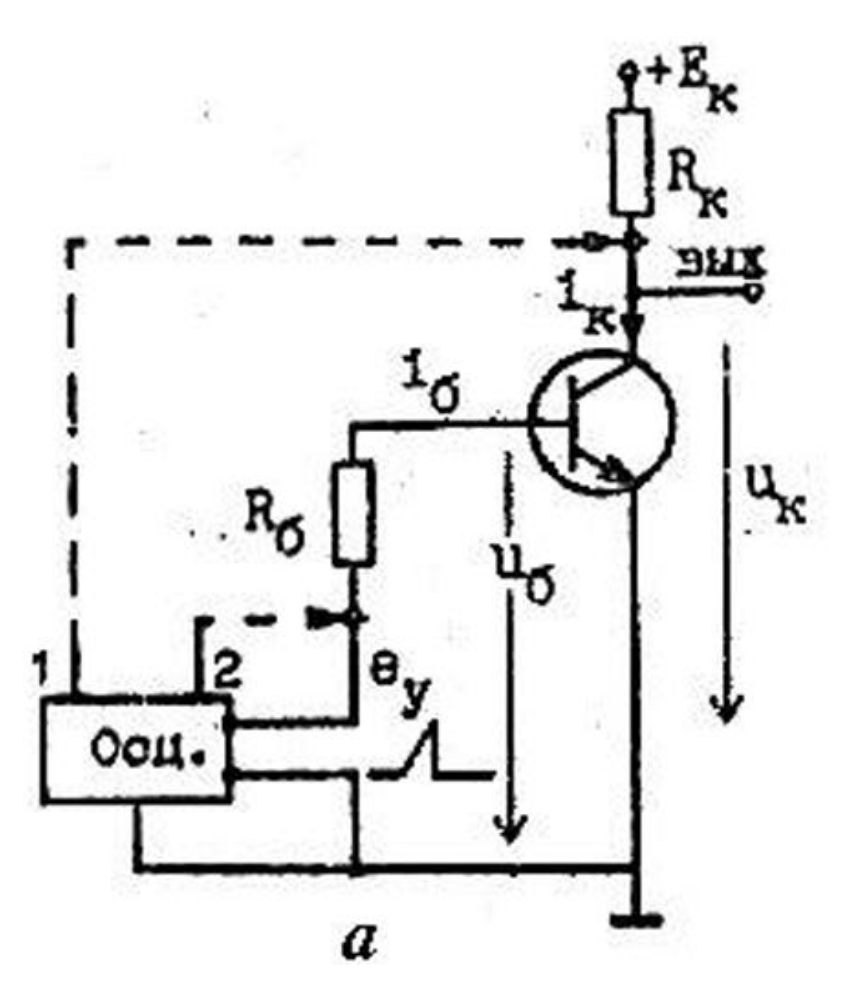
\includegraphics[width=0.4\textwidth]{18-1.png}
	\caption{Схема транзисторного ключа}
\end{figure}

Характеристики устройств:

\[
R_K = 1 \, \text{кОм}
\]
\[
R_G = 10 \, \text{кОм}
\]

В результате на осциллографе была получена следующая передаточная характеристика ключа-инвертора (рис. 2). В качестве управляющего напряжения \( e_y \) мы использовали пилообразное напряжение развёртки.

\begin{figure}[htpb]
	\centering
	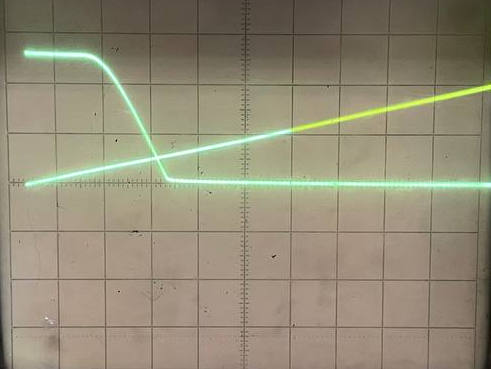
\includegraphics[width=0.5\textwidth]{18-2.jpg}
	\caption{Передаточная характеристика тразисторного ключа}
\end{figure}

1.2. В результате получились следующие значения крутизны передаточной характеристики \(\frac{du_k}{de_y}\), напряжения отсечки \( u_{60} \) и выходных напряжений \( u_{k0} \) и \( u_{kш} \), соответствующих областям отсечки и насыщения (таблица 1):

\begin{table}[h]
	\centering
	\begin{tabular}{|c|c|c|c|}
		\hline
		\(\frac{du_k}{de_y}\) & \(u_{60}\), В & \(u_{k0}\), В & \(u_{kш}\), В \\ \hline
		-6.67 & 0.7 & 5.2 & 0.2 \\ \hline
	\end{tabular}
	\caption{Значения крутизны характеристики, напряжения отсечки и выходных напряжений}
\end{table}

1.3. По значению крутизны передаточной характеристики находим коэффициент передачи тока базы транзистора:

\[
B = \frac{du_k}{de_y} \cdot \frac{R_G}{R_K} = 6.67 \cdot \frac{10 \, \text{кОм}}{1 \, \text{кОм}} = 66,7
\]

1.4. После мы подали на вход ключа управляющее напряжение \(e_y\) – прямоугольные колебания (меандр) с высокой частотой повторения: 200 кГц. Для амплитуд входных импульсов \(E_y = 7 \, \text{В}\) и \(E_y = 12.2 \, \text{В}\) получили осциллограммы управляющего и выходного напряжений, рис.3 соответственно.

\begin{figure}[htpb]
	\centering
	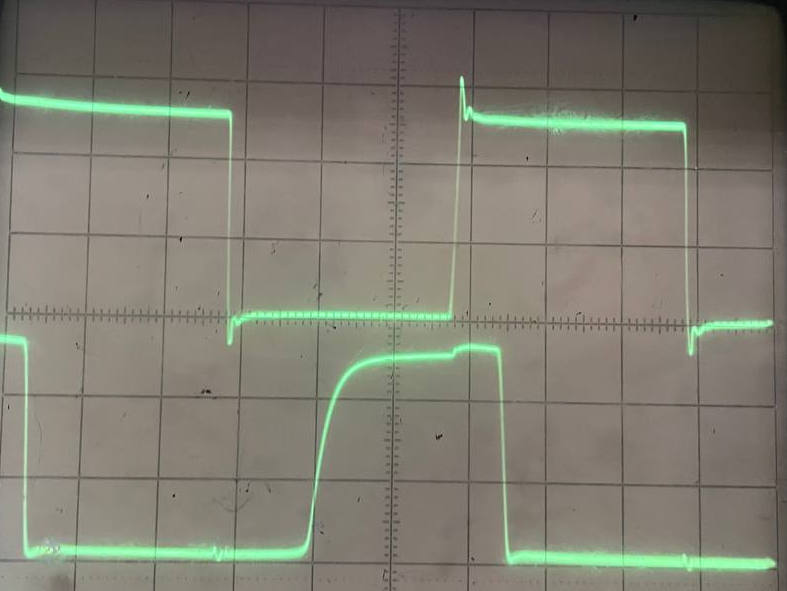
\includegraphics[width=0.5\textwidth]{18-3.jpg}
	\caption{Осцилограмма управляющего напряжения для $E_y = 7$ В}
\end{figure}

Сравним параметры, характеризующие инерционность ключа. Ими являются \( t_3 \) – время задержки включения транзистора (время подготовки), \( t_n \) – длительность включения, \( t_p \) – время рассасывания (время задержки выключения) и \( t_\phi \) – длительность выключения.

Параметры для \( E_y = 7 \, \text{В} \):

\begin{table}[h]
	\centering
	\begin{tabular}{|c|c|c|c|}
		\hline
		\( t_3, \, \text{мкс} \) & \( t_n, \, \text{мкс} \) & \( t_p, \, \text{мкс} \) & \( t_\phi, \, \text{мкс} \) \\ \hline
		0.6 & 0.5 & 0.3 & 0.4 \\ \hline
	\end{tabular}
\end{table}

Параметры для \( E_y = 12.2 \, \text{В} \):

\begin{table}[h]
	\centering
	\begin{tabular}{|c|c|c|c|}
		\hline
		\( t_3, \, \text{мкс} \) & \( t_n, \, \text{мкс} \) & \( t_p, \, \text{мкс} \) & \( t_\phi, \, \text{мкс} \) \\ \hline
		0.4 & 0.25 & 0.65 & 0.45 \\ \hline
	\end{tabular}
\end{table}

Из полученных выше результатов можно сделать следующие выводы. Время задержки включения транзистора \( t_3 \) уменьшается с повышением перепада входного напряжения \( E_y \). Также с повышением перепада входного напряжения \( E_y \) процесс отпирания, характеризуемый длительностью включения \( t_n \), заметно ускоряется. Время рассасывания \( t_p \) существенно увеличилось и заметно превышает остальные характеристики. Длительность выключения \( t_\phi \) немного увеличилась.

\subsubsection*{Триггер Шмитта}

2.1. Мы собрали триггер Шмитта, установив резисторы \( R_K=1 \, \text{кОм}, \, R_G=10 \, \text{кОм}, \, R_C: 10 \, \text{кОм} \) и 100 кОм (рис. 4).

\begin{figure}[htpb]
	\centering
	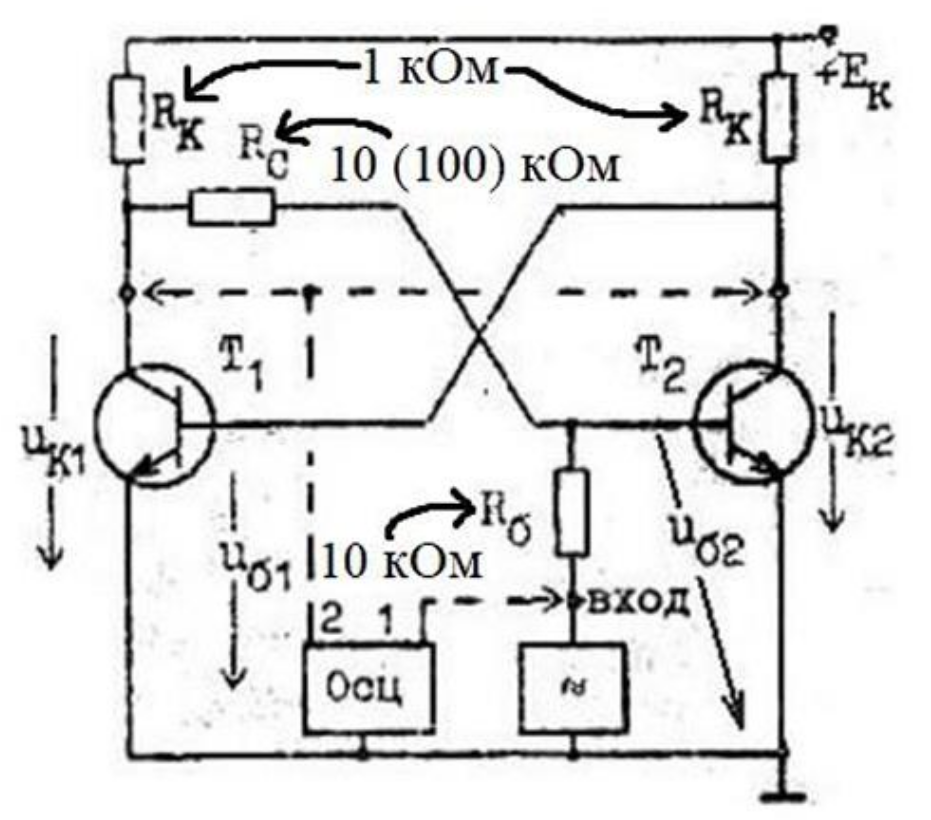
\includegraphics[width=0.4\textwidth]{18-4.png}
	\caption{Схема триггера Шмитта}
\end{figure}

Характеристики устройств:

\[
R_K = 1 \, \text{кОм}
\]
\[
R_G = 10 \, \text{кОм}
\]
\[
R_C: 10 \, \text{кОм} \, \text{и} \, 100 \, \text{кОм}
\]

2.2. В результате на осциллографе были получены следующие передаточные характеристики триггера Шмитта для прямого и инверсного выходов при \( R_C = 10 \, \text{кОм}, \, \text{рис.5}\) соответственно:

\begin{figure}[htpb]
	\centering
	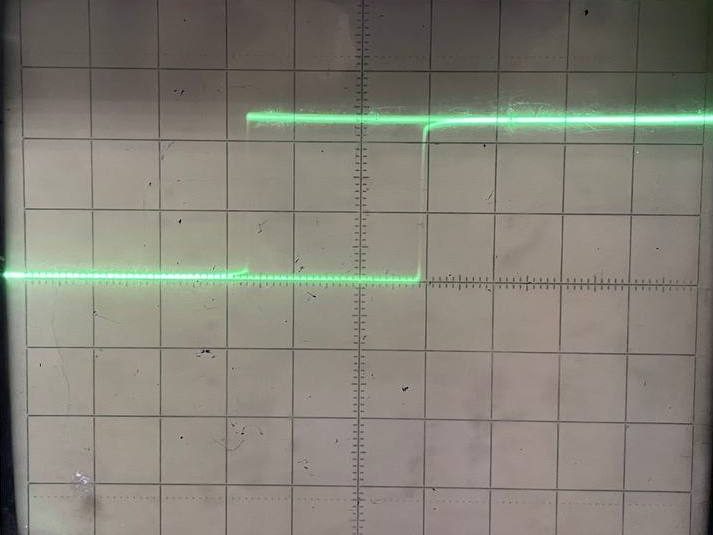
\includegraphics[width=0.5\textwidth]{18-5.jpg}
	\caption{Передаточная характеристика триггера Шмитта для прямого выхода при $R_c = 10\text{кОм}$}
\end{figure}

Значения уровней потенциалов и порогов срабатывания для прямого выхода при \( R_C = 10 \, \text{кОм} \):

\begin{table}[h]
	\centering
	\begin{tabular}{|c|c|c|c|}
		\hline
		\( U_1^0, B \) & \( U_1^1, B \) & \( E^0, B \) & \( E^1, B \) \\ \hline
		0.2 & 4.8 & -2.9 & 1.5 \\ \hline
	\end{tabular}
\end{table}

Значения уровней потенциалов и порогов срабатывания для инверсного выхода при \( R_C = 10 \, \text{кОм} \):

\begin{table}[h]
	\centering
	\begin{tabular}{|c|c|c|c|}
		\hline
		\( U_2^0, MB \) & \( U_2^1, MB \) & \( E^0, B \) & \( E^1, B \) \\ \hline
		40 & 720 & -2.9 & 1.5 \\ \hline
	\end{tabular}
\end{table}

Также были получены следующие передаточные характеристики триггера Шмитта для прямого и инверсного выходов при \( R_C = 100 \, \text{кОм} \), рис.6 соответственно:

\begin{figure}[htpb]
	\centering
	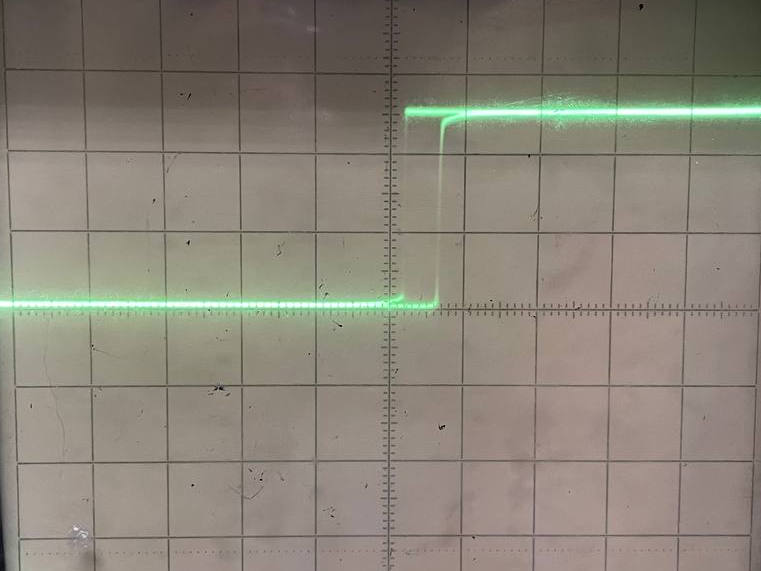
\includegraphics[width=0.5\textwidth]{18-6.jpg}
	\caption{Передаточная характеристика триггера Шмитта для прямого выхода при $R_c = 100\text{кОм}$}
\end{figure}

Значения уровней потенциалов и порогов срабатывания для прямого выхода \( R_C = 100 \, \text{кОм} \):

\begin{table}[h]
	\centering
	\begin{tabular}{|c|c|c|c|}
		\hline
		\( U_1^0, B \) & \( U_1^1, B \) & \( E^0, B \) & \( E^1, B \) \\ \hline
		0.2 & 5.2 & 0.6 & 1.1 \\ \hline
	\end{tabular}
\end{table}

Значения уровней потенциалов и порогов срабатывания для инверсного выхода при \( R_C = 100 \, \text{кОм} \):

\begin{table}[h]
	\centering
	\begin{tabular}{|c|c|c|c|}
		\hline
		\( U_2^0, MB \) & \( U_2^1, MB \) & \( E^0, B \) & \( E^1, B \) \\ \hline
		80 & 720 & 0.6 & 1.1 \\ \hline
	\end{tabular}
\end{table}

В случае для \( R_C = 100 \, \text{кОм} \) разность \( E^1 - E^0 = 0.5 \, \text{B} \), и она значительно уменьшилась по сравнению со случаем для \( R_C = 10 \, \text{кОм} \), для которого разность \( E^1 - E^0 = 4.4 \, \text{B} \). Это вызвано тем, что увеличение сопротивления \( R_C \) влияет на работу транзистора \( T_2 \), уменьшая ток через его коллектор и ослабляя обратную связь.

Также можно заметить, что в обоих случаях напряжение \( U_2^1 \) заметно меньше \( U_1^1 \). Это связано с тем, что состояния транзисторов \( T_1 \) и \( T_2 \) не являются полностью симметричными из-за различий в их нагрузках и обратных связях. Когда \( T_2 \) открыт, его коллекторное напряжение \( U_2^1 \) падает сильнее, чем \( U_1^1 \), из-за влияния \( R_C \) и асимметрии схемы.

2.3. Далее мы получили следующую осциллограмму входного \( e_y \) и выходного \( u_{kx1} \) напряжений триггера, работающего как формирователь прямоугольных импульсов при \( R_C = 10 \, \text{кОм} \) (рис. 7):

\begin{figure}[htpb]
	\centering
	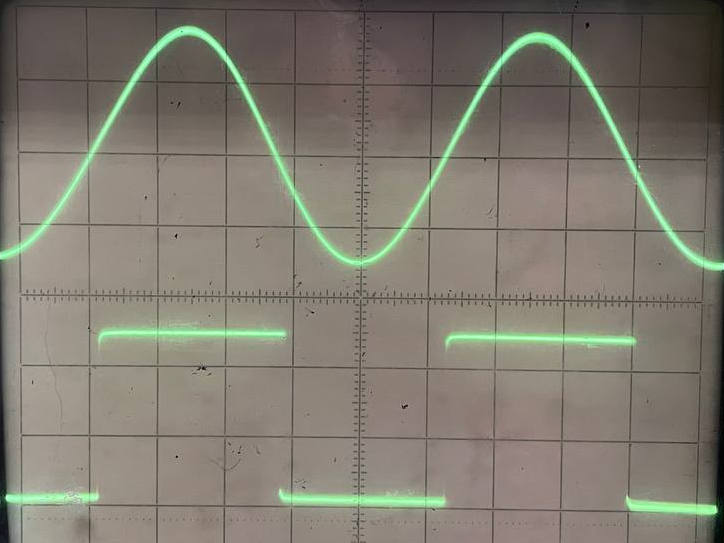
\includegraphics[width=0.5\textwidth]{18-7.jpg}
	\caption{Формирование прямоугольного напряжения на выходе триггера Шмитта}
\end{figure}

Значения уровней потенциалов и порогов срабатывания:

\begin{table}[h]
	\centering
	\begin{tabular}{|c|c|c|c|}
		\hline
		\( U_1^0, B \) & \( U_1^1, B \) & \( E^0, B \) & \( E^1, B \) \\ \hline
		0.2 & 4.8 & -3 & 2 \\ \hline
	\end{tabular}
\end{table}

\newpage

\subsubsection*{Ждущий мультивибратор}

3.1. Мы собрали схему ждущего мультивибратора (рис. 8).

\begin{figure}[htpb]
	\centering
	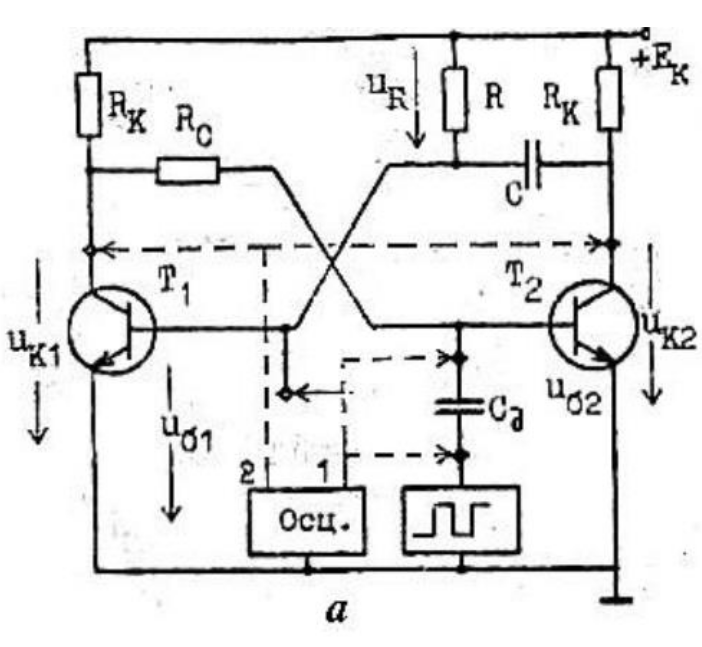
\includegraphics[width=0.4\textwidth]{18-8.png}
	\caption{Схема исследования ждущего мультивибратора}
\end{figure}

Характеристики подключенных устройств:
\[
R_c = R = 10 \, \text{кОм}
\]
\[
C = 100 \, \text{нФ}
\]
\[
C_\theta = 1 \, \text{нФ}
\]
\[
R_K = 1 \, \text{кОм}
\]

3.2. Для запуска релаксатора мы использовали стандартный генератор в режиме выдачи прямоугольных импульсов (меандра) с частотой повторения 500 Гц. Чтобы превратить прямоугольное напряжение \(e_y\) в импульсное, его нужно продифференцировать. Для этого генератор с базой транзистора \(T_2\) мы соединили с конденсатором \(C_\theta = 1 \, \text{нФ}\).

\begin{figure}
	\centering
		\begin{minipage}{0.45\textwidth}
		\centering
		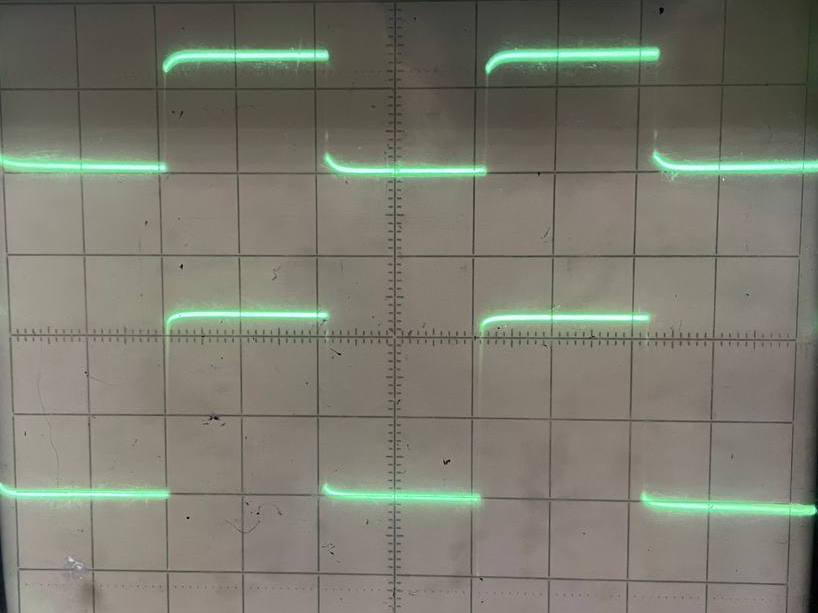
\includegraphics[width=1\linewidth]{18-9.jpg}
		\label{fig:exp_char}
	\end{minipage}
	\hfill
	\begin{minipage}{0.45\textwidth}
		\centering
		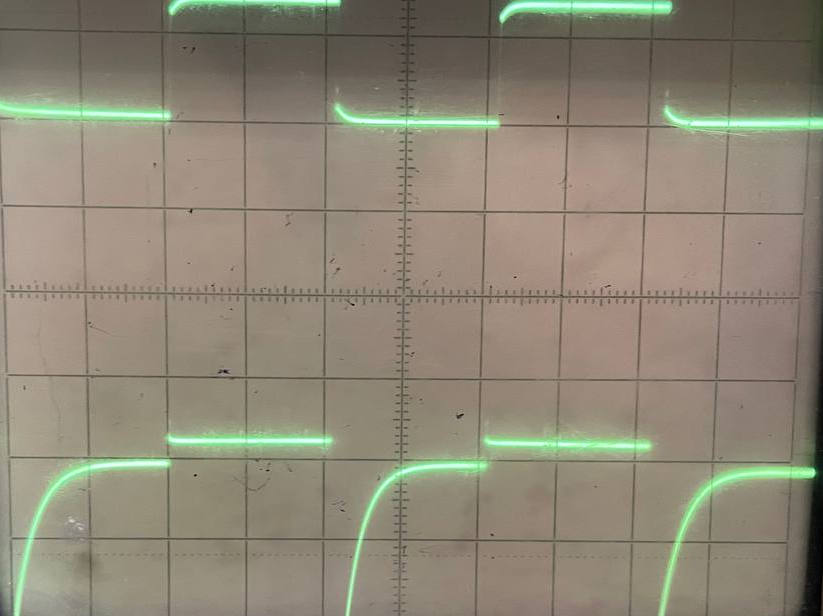
\includegraphics[width=1\linewidth]{18-10.jpg}
		\label{fig:teor_char}
	\end{minipage}
	\caption{Осциллограммы для $e_y$, $u_{\text{к1}}$, $u_{\text{к2}}$.}
\end{figure}

Мы получили осциллограммы напряжений \(e_y\), \(u_{61}\), \(u_{k1}\), \(u_{62}\), \(u_{k2}\) в одном масштабе времени.

На основе осциллограммы с рис.9 мы измерили длину импульса \(\tau = 0.7 \, \text{мс}\). Полученное значение совпадает с расчетной оценкой:

\[
\tau = 0.7RC = 0.7 \times 10 \, \text{кОм} \times 100 \, \text{нФ} = 0.7 \, \text{мс}
\]

Экспериментальное и расчетное значения длины импульса равны между собой.

3.3. Далее, мы измерили длину импульса для \(u_{к1}\) при разных частотах меандра.

\begin{table}[h]
	\centering
	\begin{tabular}{|c|c|}
		\hline
		Частота \( \nu \), кГц & Длина импульса \( \tau \), мс \\ \hline
		0.2 & 0.64 \\ \hline
		1 & 0.5 \\ \hline
		2 & 0.25 \\ \hline
	\end{tabular}
\end{table}

На основе полученных данных можно сделать вывод, что с увеличением частоты сигнала уменьшалась длина импульса. Это вызвано тем, что при окончании входного импульса происходит «опрокидывание», и при высокой частоте запуска конденсатор \(C\) не успевает полностью зарядиться или разрядиться за время между импульсами, и как следствие приводит к сокращению длительности выходного импульса.

\subsubsection*{Автоколебательный мультивибратор}

4.1. Мы собрали схему автоколебательного мультивибратора (рис. 13).

\begin{figure}[htpb]
	\centering
	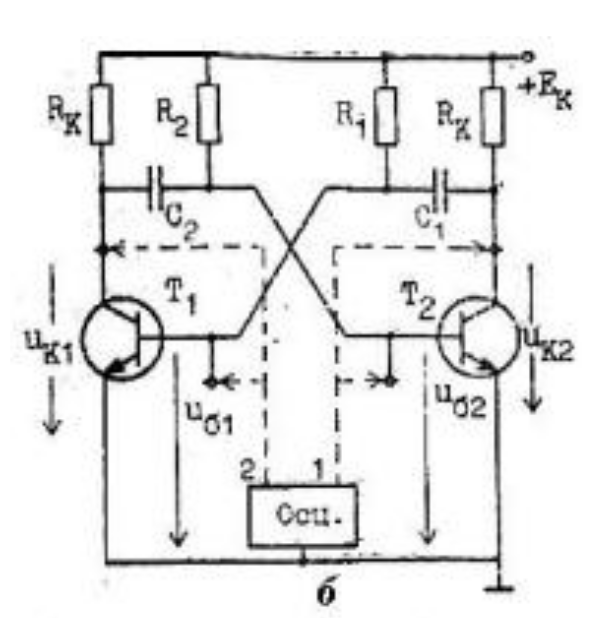
\includegraphics[width=0.4\textwidth]{18-13.png}
	\caption{Схема автоколебательного мультивибратора}
\end{figure}

Характеристики подключенных устройств:

\[
R_1 = R_2 = 10 \, \text{кОм}
\]
\[
C_1 = C_2 = 100 \, \text{нФ}
\]
\[
R_k = 1 \, \text{кОм}
\]

Используя двухлучевой режим осциллографа, получили осциллограммы напряжений \(u_{61}\), \(u_{k1}\), \(u_{k2}\) (Рис. 11 и Рис. 12).

\begin{figure}[htpb]
	\centering 
	\begin{minipage}{0.45\textwidth}
		\centering
		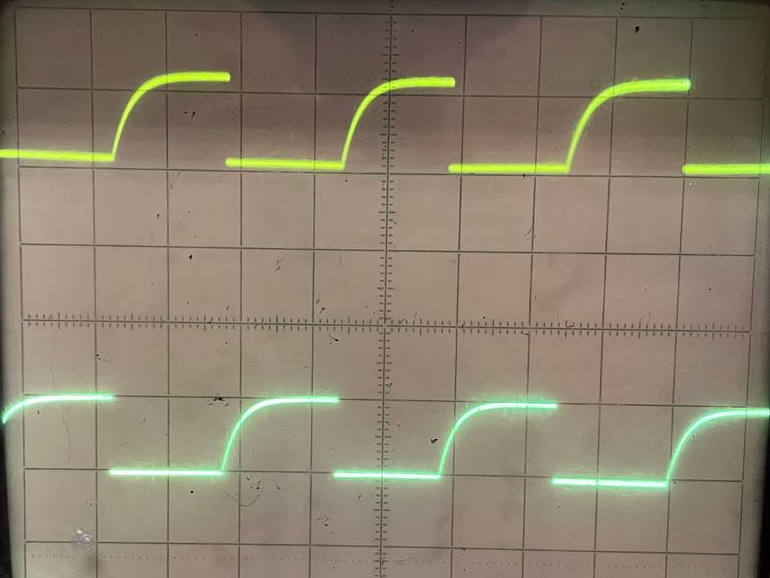
\includegraphics[width=0.9\linewidth]{18-14.jpg}
		\caption{Осциллограммы для $u_{k2}$ и $u_{k1}$}
	\end{minipage}
	\hfill
	\begin{minipage}{0.45\textwidth}
		\centering
		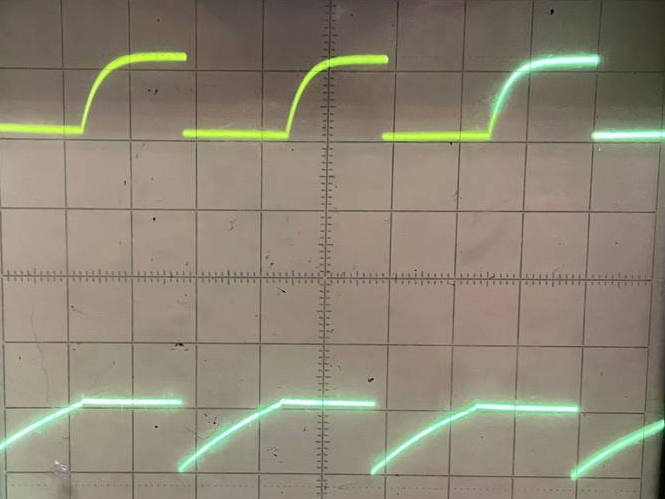
\includegraphics[width=0.9\linewidth]{18-15.jpg}
		\caption{Осциллограммы для $u_{k2}$ и $u_{\text{б1}}$}
		
	\end{minipage}
	
\end{figure}

	В представленной на рис. 10 схеме после запирания транзистора напряжение на его коллекторе не сразу достигает максимального значения $E_k$,  так как должно пройти время, чтобы зарядился конденсатор, подключенный к этому коллектору. Как итог, форма выходного напряжения не является прямоугольной.

	На основе полученных осциллограмм мы измерили импульсы по основанию:

	Для$ (U_{к1}): (\tau_1 = 0.63 \, \text{мс});$

Для \(U_{к2}\): \(\tau_2 = 0.7 \, \text{мс}\).

\subsubsection*{Вывод:}

\subsubsection*{1. Транзисторный ключ}
Из передаточной характеристики были получены следующие значения: \(\frac{du_k}{de_y} = -6.67\) – крутизна передаточной характеристики, \(B = 66.7\) – коэффициент передачи тока базы транзисторов.

При увеличении перепада входного напряжения \(E_y\) (с 7 В до 12.2 В) уменьшается время задержки включения транзистора \(t_3\) (с 0.6 мкс до 0.4 мкс) и длительность включения \(t_n\) (с 0.5 мкс до 0.25 мкс). Время рассасывания \(t_p\) (с 0.3 мкс до 0.65 мкс) увеличивается и превышает остальные характеристики. Длительность выключения увеличивается \(t_\phi\) (с 0.4 мкс до 0.45 мкс).

\subsubsection*{2. Триггер Шмитта}
При увеличении сопротивления коллектора \(R_C\) с 10 кОм до 100 кОм разность пороговых напряжений \(E^1 - E^0\) существенно уменьшилась (с 4.4 В до 0.5 В). Это связано с изменением режима работы транзистора и ослаблением обратной связи. В обоих случаях напряжение \(U_2^1\) заметно меньше \(U_1^1\), так как система не симметрична.

\subsubsection*{3. Ждущий мультивибратор}
Мы получили длину импульса \(\tau = 0.7 \, \text{мс}\), которая совпадает с расчетным значением.

С увеличением частоты входного сигнала уменьшалась длина выходного импульса из-за недостаточного заряда/разряда конденсатора между импульсами.

\subsubsection*{4. Автоколебательный мультивибратор}
Полученные осциллограммы показали, что выходное напряжение не является строго прямоугольным из-за процессов заряда и разряда конденсаторов. Измеренные длительности импульсов по основанию (\(\tau_1=0.63 \, \text{мс}\) и \(\tau_2=0.7 \, \text{мс}\)).

\end{document}